\documentclass[
]{jss}

\usepackage[utf8]{inputenc}

\providecommand{\tightlist}{%
  \setlength{\itemsep}{0pt}\setlength{\parskip}{0pt}}

\author{
Emiliano Villicaña García\\UNAM FE \And Eduardo Aguilar Vázquez\\UNAM FE
}
\title{Proyecto Final}

\Plainauthor{Emiliano Villicaña García, Eduardo Aguilar Vázquez}
\Plaintitle{Proyecto Final}
\Shorttitle{Probabilidad y Estadística 2020-2}

\Abstract{

}


%% publication information
%% \Volume{50}
%% \Issue{9}
%% \Month{June}
%% \Year{2012}
%% \Submitdate{}
%% \Acceptdate{2012-06-04}

\Address{
    }


% Pandoc header

\usepackage{amsmath}

\begin{document}

\hypertarget{instrucciones}{%
\section{Instrucciones}\label{instrucciones}}

\#\#El proyecto constará de dos partes con una duración de una semana
respectivamente. Para la primera parte deberán elegir una pregunta,
misma que se responderá a través de los datos de instancias oficiales.
Así como crear una gráfica sencilla que represente la pregunta que
eligieron. Para la segunda parte, harán la presentaciónn de su pantalla
y nos describirán su código. Veamos las instrucciones de la Parte 1:

\hypertarget{deberuxe1s-responder-una-pregunta-de-tu-interuxe9s-la-cual-deberuxe1-sustentarse-con-datos-de-instancias-oficiales.-algunos-ejemplos-son}{%
\subsection{Deberás responder una pregunta de tu interés, la cual deberá
sustentarse con datos de instancias oficiales. Algunos ejemplos
son:}\label{deberuxe1s-responder-una-pregunta-de-tu-interuxe9s-la-cual-deberuxe1-sustentarse-con-datos-de-instancias-oficiales.-algunos-ejemplos-son}}

\begin{itemize}
\item ¿Cuánto creció el desempleo?
\item ¿Cuál fue el número de contagiados de COVID-19 en el mes de Marzo?
\item ¿Qué producto se vende más en el negocio de mis papás?
\item ¿Cuál es el país con menor brecha de género?
\end{itemize}

\hypertarget{necesitaruxe1s-que-existan-datos-e-importarlos.}{%
\subsection{Necesitarás que existan datos e
importarlos.}\label{necesitaruxe1s-que-existan-datos-e-importarlos.}}

Recuerden la importancia del manejo de datos, siempre los vamos a
necesitar para trabajar, es nuestra herramienta para darle vida a la
teoría, por ello es recomendable que sepan dónde encontrar rapidamente
la información y que tenga un formato sencillo (.xlsx, .csv, .txt) o de
la API de Banco Mundial.

\hypertarget{describir-sus-datos-y-hacer-transformaciones}{%
\subsection{Describir sus datos y hacer
transformaciones}\label{describir-sus-datos-y-hacer-transformaciones}}

Una vez que tengan los datos deberán describirlos contestando las
siguientes preguntas:

\begin{itemize}
\item ¿Cuántos datos tengo?
\item ¿Qué tipo de variables son?
\item ¿Están en el formato correcto?
\item ¿Tengo errores de captura o datos imposibles?
\end{itemize}

Dependiendo de su pregunta necesitarán crear variables, agrupar,
filtrar, obtener estadística descriptiva, etc.

\hypertarget{realicen-una-gruxe1fica-sencilla}{%
\subsection{Realicen una gráfica
sencilla}\label{realicen-una-gruxe1fica-sencilla}}

Dependiendo del tipo de relación o variables que tengan, deberán elegir
la gráfica que mejor represente su pregunta.

\hypertarget{ejemplo.}{%
\section{Ejemplo.}\label{ejemplo.}}

Este será uno sencillo, es recomendable empezar con información que ya
sabemos para validar el procedimiento. ¿Cuántos confirmados tenemos de
COVID-19 al día de hoy? Sabemos que hay 71,105 veremos si concuerda.

\begin{CodeChunk}

\begin{CodeInput}
R> library(tidyverse)
R> library(covidMex)
\end{CodeInput}
\end{CodeChunk}

\begin{CodeChunk}

\begin{CodeInput}
R> df <- covidOfficialMx()
\end{CodeInput}

\begin{CodeOutput}
Warning in covidMex::GetFromSSA(date = date, neat = neat): Please keep in mind
that the official report on Covid-19 cases has not a version control system or
whatsover, therefore it's still difficult to match a specific date to a version
of the report. The latest version available will be downloaded (it can be from
yesterday's).
\end{CodeOutput}

\begin{CodeInput}
R> df %>%
R+   filter(RESULTADO == 'Positivo a SARS-CoV-2') %>% ## Esto debería ser una etiqueta como 1,2,3
R+   tally()
\end{CodeInput}

\begin{CodeOutput}
# A tibble: 1 x 1
      n
  <int>
1 71105
\end{CodeOutput}
\end{CodeChunk}

Como el dato concuerda podemos adentrarnos más. De los confirmados
¿Cuántos son hombres y cuántos son mujeres?

\begin{CodeChunk}

\begin{CodeInput}
R> df %>%
R+   filter(RESULTADO == 'Positivo a SARS-CoV-2') %>% ## De verdad, esto debería ser una etiqueta como 1,2,3
R+   group_by(SEXO) %>%
R+   tally()
\end{CodeInput}

\begin{CodeOutput}
# A tibble: 2 x 2
  SEXO          n
  <fct>     <int>
1 Femenino  30642
2 Masculino 40463
\end{CodeOutput}
\end{CodeChunk}

De los confirmados por sexo ¿Cuál es la distribución de edad?

\begin{CodeChunk}

\begin{CodeInput}
R> confirmados <- df %>%
R+   filter(RESULTADO == 'Positivo a SARS-CoV-2')
R> mu <- confirmados %>% group_by(SEXO) %>% summarise(media = mean(EDAD))
R> ggplot(confirmados,aes(x = EDAD, col = SEXO)) + geom_bar(stat = 'count', position = 'dodge') +
R+    geom_vline(data = mu, aes(xintercept=media, color=SEXO),
R+              linetype="dashed") + ## Ahora la hacemos bonita
R+   theme_linedraw() + labs(
R+     title = "Distribución de edad de los confirmados de COVID-19 por sexo",
R+     subtitle = 'Elaborada como ejemplo para la práctica de \nla clase de Probabilidad y Estadística, UNAM FE',
R+     caption = 'Elaboración propia con datos de la Secretaría de Salud',
R+     x = 'Edad',
R+     y = 'Distribución' )
\end{CodeInput}


\begin{center}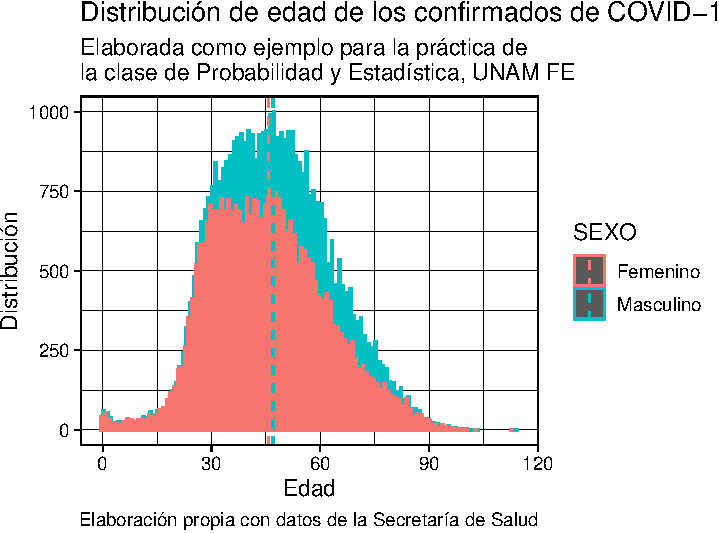
\includegraphics{PracticaFinal_files/figure-latex/unnamed-chunk-4-1} \end{center}

\end{CodeChunk}



\end{document}

